Los modelos lineales surgieron con el propósito de estructurar el desarrollo de software, que inicialmente carecía de orden. Constituyen la base de la ingeniería de software \cite{pressmanIngenieriaSoftwareEnfoque2013}. En ellos, el desarrollo se separa en etapas que se llevan a cabo de forma secuencial. Si bien en el presente se favorecen sistemas más interactivos, los modelos lineales son la base en la que se construye el desarrollo del software.
%
%
\subsection{Modelo en cascada}
\par El modelo en cascada es el más básico de las SDLC. En este modelo, se avanza por cada etapa secuencialmente, desde la concepción del producto hasta su entrega \cite{pressmanIngenieriaSoftwareEnfoque2013,sStudySoftwareDevelopment2017,dwivediComparativeStudyVarious2022}. Cada etapa es considerada un módulo independiente, y sólo se avanza cuando se ha completado \cite{dwivediComparativeStudyVarious2022}.
\par Durante la primera etapa, se establecen los requerimientos a completar, además de un plan de acción que engloba a todas las actividades de cada módulo. Cada fase genera uno o más documentos que permiten avanzar a la siguiente fase una vez que son aprobados \cite{sommervilleIngenieriaSoftware9a2011}. Este proceso se continúa hasta completar el software.
%
\begin{figure}[h]
  \centering
  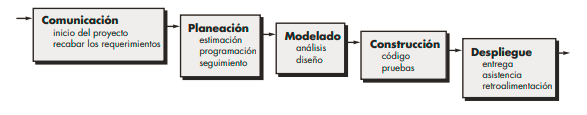
\includegraphics[scale=0.5]{image3.png}
  \caption{Modelo en cascada. Extraída de \cite{pressmanIngenieriaSoftwareEnfoque2013}.}
  \label{fig:x Modelo en cascada}
\end{figure}
%
\par Este modelo es el más antiguo de la ingeniería del software, ideado inicialmente en 1956 por el autor Herbert Bennington y luego modificado por Winston Royce en 1970 [17].
El modelo original, provisto por Bennington, recomendaba desarrollar el software en etapas separadas. Royce luego reconoció que en situaciones reales podrían aparecer dificultades inesperadas, por lo que su versión de cascada añade puntos de retorno en cada etapa, en caso de que sea necesario revisitar un estado anterior \cite{rupareliaSoftwareDevelopmentLifecycle2010,royceManagingDevelopmentLarge1970}. Sin embargo, la mayoría de las organizaciones aplican este modelo de forma estrictamente lineal \cite{pressmanIngenieriaSoftwareEnfoque2013}.
\begin{figure}[h]
  \centering
  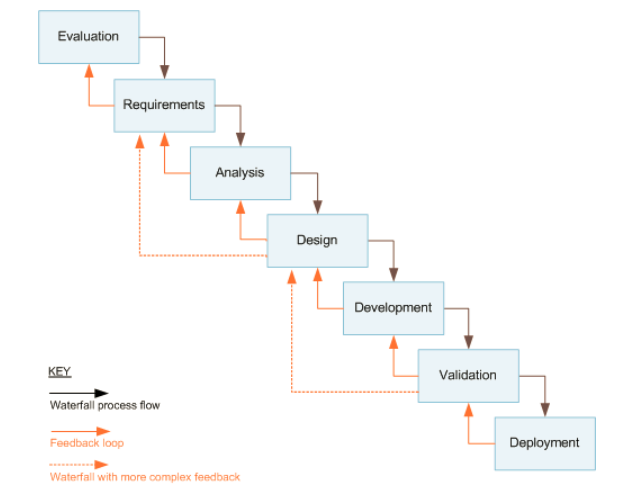
\includegraphics[scale=0.5]{image2.png}
  \caption{Modelo en cascada propuesto por Bennington. Extraída de \cite{rupareliaSoftwareDevelopmentLifecycle2010}.}
  \label{fig:x Modelo en cascada propuesto por Bennington}
\end{figure}
\subsubsection{Ventajas}
\begin{itemize}
  \item Útil para proyectos pequeños donde haya fases claramente definidas.
  \item Cada fase genera un producto entregable.
  \item Documentación extensa de los procesos y resultados.
\end{itemize}
\subsubsection{Desventajas}
\begin{itemize}
  \item Mucha resistencia al cambio, hace que sea difícil implementar en situaciones reales donde los requisitos varían constantemente.
  \item Los requerimientos se establecen al principio y no se pueden cambiar.
  \item No se obtiene un producto funcional hasta el final del proceso.
\end{itemize}
%
%
\subsection{Modelo en V}
\par El modelo en V, también conocido como el modelo de validación y verificación, es una variación del modelo en cascada \cite{rupareliaSoftwareDevelopmentLifecycle2010} donde se añade una segunda lista de etapas en dirección contraria, que retorna feedback para cada uno de los módulos llevados a cabo durante el desarrollo \cite{pressmanIngenieriaSoftwareEnfoque2013,rupareliaSoftwareDevelopmentLifecycle2010,dwivediComparativeStudyVarious2022}.
%
\begin{figure}[h]
  \centering
  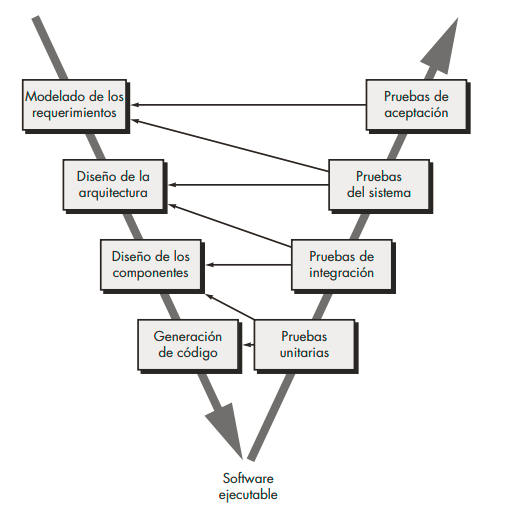
\includegraphics[scale=0.5]{image7.png}
  \caption{Modelo en cascada V. Extraída de \cite{pressmanIngenieriaSoftwareEnfoque2013}.}
  \label{fig:x modelo en v}
\end{figure}
%
\subsubsection{Ventajas}
\begin{itemize}
    \item Se adapta bien en proyectos con requerimientos claramente definidos.
    \item El proceso de validación genera un producto robusto.
\end{itemize}
\subsubsection{Desventajas}
\begin{itemize}
    \item Al igual que el método en cascada, es muy resistente al cambio de requerimientos.
    \item El proceso de validación no se realiza hasta que el software esté completado.
\end{itemize}